% Provenance (never printed): see sources/outline_sources.md (Year 1: physical and chemical
% weathering; hydrolysis and its degrees; the ionic-potential diagram; clay minerals and
% climate; silicate weathering and carbon dioxide). Exercise and problem values in the Book 3
% scratch calculator calc/ch19.py; figure data from figdata/bachelor-1/ionic_potential.py and
% hydrolysis.py. Weathering is owned by Book 1 g5; chemical weathering, hydrolysis, clay mineral
% and laterite by Book 2 g10 (re-founded here). Silicate classes and the feldspars by ch. 7;
% Bowen's series by Book 2 g11; acid--base chemistry, solubility and oxidation by the chemistry
% books; soils and their horizons by the biology books. The silicate-weathering thermostat
% belongs to the Year 2 volume (told).
\chapter{Intemperismo e argilas}\label{ch:b1:weathering-clays}

A inscrição de uma lápide antiga se apaga, as arestas vivas das letras arredondam-se em sulcos rasos, mais depressa numa pedra de mármore do que numa de ardósia. Um \omterm{def:b1:geological-maps:geological-map}{afloramento} de granito que parece tão duro quanto qualquer coisa na Terra esfarela-se na superfície numa areia granulosa, que escorre pelos dedos como grãos soltos de quartzo vítreo, \omterm{def:b1:rock-forming-minerals:groups}{feldspato} fosco e lascas de \omterm{def:b1:rock-forming-minerals:groups}{mica}. Sob as florestas dos trópicos úmidos, a rocha sólida pode jazer bem abaixo de uma terra vermelha que mantém os contornos dos \omterm{def:b1:rock-forming-minerals:mineral}{minerais} da rocha, mas pode ser cortada com uma pá. Os três são obra da água na superfície da Terra. Este capítulo escreve esse trabalho como química: quais \omterm{def:b1:rock-forming-minerals:mineral}{minerais} cedem primeiro, no que se transformam, por que alguns elementos saem com a água e outros ficam, como o clima determina o resultado, e como a lenta decomposição da rocha silicatada retira gás carbônico do ar.

\begin{recall}
O intemperismo desfaz as rochas onde elas estão (Livro 1, 5º ano). O \omterm{def:b1:weathering-clays:weathering}{intemperismo químico} transforma os \omterm{def:b1:rock-forming-minerals:mineral}{minerais}; a \omterm{def:b1:weathering-clays:hydrolysis}{hidrólise} de um \omterm{def:b1:rock-forming-minerals:groups}{feldspato} dá um \omterm{def:b1:rock-forming-minerals:mineral}{mineral} argiloso, a \omterm{def:b1:weathering-clays:clay-mineral}{caulinita}, e envia potássio e sílica aos rios; uma \omterm{def:b1:weathering-clays:laterite}{laterita} é o produto vermelho, rico em ferro e alumínio, de climas quentes e úmidos (Livro 2, 10º ano). Os silicatos são classificados pelo modo como seus tetraedros \ce{SiO4} compartilham vértices, um \omterm{def:b1:rock-forming-minerals:silicate-classes}{filossilicato} formando lâminas; os \omterm{def:b1:rock-forming-minerals:groups}{feldspatos} são silicatos de armação de sódio, potássio e cálcio, as \omterm{def:b1:rock-forming-minerals:groups}{micas} silicatos laminares com potássio entre as lâminas (\cref{def:b1:rock-forming-minerals:silicate-classes},
\cref{def:b1:rock-forming-minerals:groups}). O raio iônico de um íon depende de sua carga e de sua coordenação (\cref{ch:b1:rock-forming-minerals}). Os \omterm{def:b1:rock-forming-minerals:mineral}{minerais} cristalizam de um magma em resfriamento na ordem da série de reações de Bowen, \omterm{def:b1:rock-forming-minerals:groups}{olivina} primeiro e quartzo por último (Livro 2, 11º ano). Um ácido libera íons hidrogênio; o gás carbônico dissolvido na água forma ácido carbônico; uma oxidação é uma perda de elétrons; uma equação balanceada conserva cada elemento e a carga (os livros de química). Um solo é uma camada viva organizada em horizontes (os livros de biologia).
\end{recall}

\section{Intemperismo físico e químico}\label{sec:b1:weathering-clays:types}

Uma rocha formada em profundidade, em alta temperatura e pressão e sem água livre nem oxigênio, está fora do equilíbrio na superfície. Ela se ajusta de duas maneiras, que atuam juntas.

\begin{definition}[Intemperismo físico, intemperismo químico]\label{def:b1:weathering-clays:weathering}
O \emph{intemperismo físico}\index{intemperismo físico} é a desagregação de uma rocha no lugar em fragmentos menores, sem mudança de seus \omterm{def:b1:rock-forming-minerals:mineral}{minerais}. O \emph{intemperismo químico}\index{intemperismo químico} é a transformação dos \omterm{def:b1:rock-forming-minerals:mineral}{minerais} de uma rocha no lugar por reação com a água e as substâncias que ela carrega, sobretudo íons hidrogênio, gás carbônico dissolvido e oxigênio: alguns \omterm{def:b1:rock-forming-minerals:mineral}{minerais} se dissolvem, outros são substituídos por novos \omterm{def:b1:rock-forming-minerals:mineral}{minerais} estáveis na superfície, e parte da rocha sai em solução.
\end{definition}
% ledger: formoso:weathering

\emph{Geada.} A água a \qty{0}{\celsius} tem densidade \qty{999.87}{kg.m^{-3}}, o gelo \qty{916.72}{kg.m^{-3}}: a água se expande em \qty{9.1}{\percent} ao congelar. A velha imagem do intemperismo pela geada é a de água que congela em uma fissura fechada e a abre à força, de novo a cada degelo e congelamento. Um modelo de fissuras em granito e mármore, construído sobre a mecânica da fratura e sobre o que se conhece de solos em congelamento, põe o peso em outro lugar: a água é atraída através dos poros em direção ao gelo já existente em uma fissura, como o é em direção às lentes de gelo de um solo em congelamento, e o gelo cresce e cunha a fissura enquanto durar o congelamento. O congelamento sustentado é mais eficaz entre cerca de \qty{-4}{\celsius} e \qty{-15}{\celsius}: mais perto de zero o gelo não consegue acumular pressão suficiente, e mais frio a água não consegue mais se deslocar até ele.
% ledger: usgs:water-density, iapws:ice-density, wh85:frost

\emph{Aquecimento, descarga e sal.} O aquecimento e o resfriamento repetidos fatigam uma rocha cujos \omterm{def:b1:rock-forming-minerals:mineral}{minerais} se expandem em quantidades diferentes; um granito trazido à superfície pela erosão, aliviado do peso acima dele, expande-se e se parte em lâminas paralelas à superfície; sais que cristalizam da água em evaporação, em desertos e em costas, afastam os grãos.

O \omterm{def:b1:weathering-clays:weathering}{intemperismo físico} faz mais que quebrar a rocha: ele a abre à água.

\begin{proposition}[A superfície aberta pela fragmentação]\label{prop:b1:weathering-clays:surface}
Um cubo de lado $L$ cortado em cubos de lado $L/n$ tem $n$ vezes a área de superfície. Mais geralmente, uma massa $m$ de grãos de densidade $\rho$, todos cubos de lado $d$, tem a área de superfície $S = 6m/(\rho d)$: a superfície específica $S/m =
6/(\rho d)$ é inversamente proporcional ao tamanho do grão.
\end{proposition}

\begin{proof}
Um cubo de lado $d$ tem área $6d^2$ e massa $\rho d^3$, logo a superfície específica de cada grão, e de qualquer número deles, é $6d^2/(\rho d^3)
= 6/(\rho d)$. Cortar um cubo de lado $L$ em $n^3$ cubos de lado $L/n$ mantém a massa e divide $d$ por $n$, o que multiplica a área por $n$.
\end{proof}

Um bloco de \omterm{def:b1:rock-forming-minerals:groups}{feldspato} de densidade de cerca de \qty{2600}{kg.m^{-3}} tem uma superfície específica de \qty{0.23}{m^2.kg^{-1}} na forma de fragmentos de centímetros, e \qty{2.3}{m^2.g^{-1}} na forma de grãos micrométricos, dez mil vezes mais. As reações químicas se processam nas superfícies, de modo que uma rocha estilhaçada pela geada ou aberta ao longo de suas juntas se intemperiza quimicamente muito mais depressa que a mesma rocha intacta.
% ledger: hom:albite, hom:orthoclase

\emph{As reações químicas.} A calcita se dissolve por completo em água que carrega gás carbônico, e por isso as lápides de mármore perdem suas inscrições (Livro 2, 10º ano). O ferro(II) dos silicatos escuros é oxidado a ferro(III), que permanece como óxidos amarelo-marrons e vermelhos. O mais importante, de longe, pois os silicatos formam a maior parte da \omterm{def:b1:layered-earth:layers}{crosta}, é a \omterm{def:b1:weathering-clays:hydrolysis}{hidrólise}. Os íons hidrogênio vêm do gás carbônico, dissolvido do ar e exalado por raízes e decompositores para o solo, e dos ácidos orgânicos de plantas em decomposição: águas de superfície e de solo não poluídas têm pH entre 5.5 e 7, e a água da camada orgânica de alguns solos florestais chega a 3.5. Água, temperatura, área de superfície e acidez são, assim, os quatro controles do \omterm{def:b1:weathering-clays:weathering}{intemperismo químico}, e um clima quente e úmido com um solo espesso fornece os quatro.
% ledger: formoso:weathering

\section{A hidrólise dos silicatos}\label{sec:b1:weathering-clays:hydrolysis}

\begin{definition}[Hidrólise de um silicato]\label{def:b1:weathering-clays:hydrolysis}
A \emph{hidrólise}\index{hidrólise (de silicatos)} de um silicato é sua reação com água e íons hidrogênio, na qual os íons hidrogênio substituem os cátions metálicos, que passam à solução; parte ou todo o silício sai como ácido silícico dissolvido \ce{H4SiO4}, e o restante do \omterm{def:b1:rock-forming-minerals:mineral}{mineral} se reconstrói em um novo sólido, um \omterm{def:b1:rock-forming-minerals:mineral}{mineral} argiloso ou um hidróxido. A dissolução é incongruente: o sólido que resta não tem a composição do \omterm{def:b1:rock-forming-minerals:mineral}{mineral} atacado.
\end{definition}
% ledger: formoso:weathering

O alumínio é a chave para escrever a reação: no pH de solos e rios ele é quase insolúvel, e o produto sólido o retém todo. Tudo o mais segue daí.

\begin{method}[Balanceando uma reação de hidrólise]\label{met:b1:weathering-clays:balance}
Dados o \omterm{def:b1:rock-forming-minerals:mineral}{mineral} atacado e o produto sólido:
\begin{enumerate}
  \item Tome uma unidade de fórmula do produto, e a quantidade do \omterm{def:b1:rock-forming-minerals:mineral}{mineral} que traga o mesmo número de átomos de alumínio.
  \item O silício do \omterm{def:b1:rock-forming-minerals:mineral}{mineral} não usado pelo produto sai como \ce{H4SiO4}; os cátions metálicos não usados pelo produto saem como íons.
  \item Balanceie a carga desses cátions com íons hidrogênio à esquerda.
  \item Balanceie o oxigênio com água à esquerda.
  \item Verifique o hidrogênio: ele deve se balancear sozinho. Se não se balancear, alguma fórmula está errada.
  \item Se uma equação com coeficientes inteiros for desejada, multiplique tudo.
\end{enumerate}
\end{method}

\begin{proposition}[Hidrólise dos feldspatos]\label{prop:b1:weathering-clays:feldspars}
Com a \omterm{def:b1:weathering-clays:clay-mineral}{esmectita} beidelita \ce{Na_{0.5}Al2(Si_{3.5}Al_{0.5})O10(OH)2}
(água entre as camadas omitida), \omterm{def:b1:weathering-clays:clay-mineral}{caulinita} \ce{Al2Si2O5(OH)4} e gibbsita
\ce{Al(OH)3} como produtos,
\begin{align*}
&\ce{5 NaAlSi3O8 + 4 H+ + 16 H2O -> 2 Na_{0.5}Al2(Si_{3.5}Al_{0.5})O10(OH)2 + 4 Na+ + 8 H4SiO4},\\ % ce-unbalanced-ok: decimal subscripts the checker cannot read; balance tested in tests/bachelor-1/test_weathering_clays.py
&\ce{2 NaAlSi3O8 + 2 H+ + 9 H2O -> Al2Si2O5(OH)4 + 2 Na+ + 4 H4SiO4},\\
&\ce{NaAlSi3O8 + H+ + 7 H2O -> Al(OH)3 + Na+ + 3 H4SiO4},\\
&\ce{CaAl2Si2O8 + 2 H+ + H2O -> Al2Si2O5(OH)4 + Ca^2+}.
\end{align*}
A albita perde \qty{80}{\percent} de seu sódio e $8/15$ de seu silício para a solução na primeira reação, todo o seu sódio e $2/3$ de seu silício na segunda, e tudo de ambos na terceira. A anortita perde todo o seu cálcio e nenhum de seu silício.
\end{proposition}
% ledger: webmineral:clays-b19, hom:albite, hom:anorthite

\begin{proof}
Aplique o método. Primeira reação: duas unidades de beidelita contêm $2\times2.5 = 5$ alumínios, o alumínio de 5 albitas; os 15 silícios da albita menos os $2\times3.5 = 7$ do produto deixam 8 \ce{H4SiO4}; os 5 sódios menos 1 deixam
4 \ce{Na+}, balanceados por 4 \ce{H+}; oxigênio, $40 + w$ à esquerda e $24 + 32 =
56$ à direita, dá $w = 16$; hidrogênio, $4 + 32 = 36$ e $4 + 32 = 36$,
confere. Segunda: 2 albitas dão os 2 alumínios da \omterm{def:b1:weathering-clays:clay-mineral}{caulinita}, $6 - 2 = 4$
\ce{H4SiO4}, 2 \ce{Na+} e 2 \ce{H+}; oxigênio $16 + w = 9 + 16$ dá $w = 9$;
hidrogênio $2 + 18 = 20 = 4 + 16$. Terceira: uma albita, três ácidos silícicos, um
\ce{Na+} e um \ce{H+}; oxigênio $8 + w = 3 + 12$ dá $w = 7$; hidrogênio
$1 + 14 = 15 = 3 + 12$. Quarta: os 2 alumínios e 2 silícios da anortita são
exatamente os da \omterm{def:b1:weathering-clays:clay-mineral}{caulinita}, nenhum ácido silícico sai, \ce{Ca^2+} precisa de 2 \ce{H+};
oxigênio $8 + w = 9$ dá $w = 1$; hidrogênio $2 + 2 = 4$. As frações exportadas são os íons em solução sobre os átomos no \omterm{def:b1:rock-forming-minerals:mineral}{mineral}: $4/5$ e $8/15$, depois $2/2$ e $4/6$, depois $1/1$ e $3/3$.
\end{proof}

A mesma albita pode, assim, dar três sólidos diferentes, e qual deles ela dá depende de quanta água atravessa a rocha e carrega os produtos para longe: pouca água, e muito da sílica e alguns cátions permanecem para construir uma \omterm{def:b1:weathering-clays:clay-mineral}{esmectita}; mais água, e apenas a sílica suficiente para a \omterm{def:b1:weathering-clays:clay-mineral}{caulinita} permanece; muita água, e a sílica sai por completo.

\begin{definition}[Bissialitização, monossialitização, alitização]\label{def:b1:weathering-clays:hydrolysis-degree}
O grau da \omterm{def:b1:weathering-clays:hydrolysis}{hidrólise} dos silicatos recebe o nome de seu produto. A \emph{bissialitização}\index{bissialitização} forma argilominerais 2:1, como as \omterm{def:b1:weathering-clays:clay-mineral}{esmectitas}, com cerca de dois átomos de silício por alumínio; parte dos cátions permanece neles. A \emph{monossialitização}\index{monossialitização} forma argilominerais 1:1, a \omterm{def:b1:weathering-clays:clay-mineral}{caulinita}, com um silício por alumínio; todos os cátions alcalinos e alcalino-terrosos saem. A \emph{alitização}\index{alitização} remove o silício por completo e deixa hidróxido de alumínio, a gibbsita.
\end{definition}
% ledger: pedron:stages, formoso:weathering

O grau atingido é uma questão de clima antes de tudo, pela chuva e pela temperatura, e depois da drenagem do perfil. Onde a água é pouco renovada, um granito perde grande parte de seu sódio e cálcio, potássio mais
lentamente, e apenas parte de sua sílica: seus \omterm{def:b1:rock-forming-minerals:groups}{feldspatos} se transformam em argilas 2:1, e muito quartzo resta; a rocha se desfaz em uma areia de quartzo, \omterm{def:b1:rock-forming-minerals:groups}{mica} e \omterm{def:b1:rock-forming-minerals:groups}{feldspato} meio intemperizado misturados a argila. Sob as chuvas intensas dos trópicos úmidos, mais de \qty{2000}{mm} por ano, os cátions e a sílica são lixiviados muito mais, e forma-se a \omterm{def:b1:weathering-clays:clay-mineral}{caulinita}, com Si/Al = 1. Onde a lixiviação é mais intensa, até a sílica da \omterm{def:b1:weathering-clays:clay-mineral}{caulinita} sai, e resta a gibbsita.
% ledger: pedron:stages, goldich:1938, formoso:laterite

\begin{omfigure}
\begin{tikzpicture}[font=\small]
% fractions of albite's Na and Si exported by the three degrees (figdata/bachelor-1/hydrolysis.py)
\begin{axis}[width=10.5cm, height=6cm, ybar, bar width=0.5cm, ymin=0, ymax=112,
    xmin=0.45, xmax=3.55, xtick={1,2,3},
    xticklabels={{bissialitização\\ a beidelita\\ (Si/Al = 1.4)}, {monossialitização\\ a caulinita\\ (Si/Al = 1)}, {alitização\\ a gibbsita\\ (Si/Al = 0)}},
    xticklabel style={align=center, font=\footnotesize},
    ylabel={exportado em solução (\si{\percent})}, ytick={0,20,...,100},
    legend style={at={(0.5,1.03)}, anchor=south, font=\footnotesize, legend columns=2, draw=none},
    nodes near coords={\pgfmathprintnumber[fixed,precision=0]{\pgfplotspointmeta}}, every node near coord/.append style={font=\scriptsize},
    enlarge x limits=false]
  \addplot[fill=omThm!60, draw=omThm!80!black] table[x=degree, y=Na] {figdata/out/bachelor-1-hydrolysis-degrees.dat};
  \addplot[fill=omDef!55, draw=omDef!80!black] table[x=degree, y=Si] {figdata/out/bachelor-1-hydrolysis-degrees.dat};
  \legend{sódio, silício}
\end{axis}
\end{tikzpicture}

{\small Os três graus de \omterm{def:b1:weathering-clays:hydrolysis}{hidrólise} da albita: a porcentagem de seu sódio e de seu silício levados embora em solução, calculada a partir das reações balanceadas, e a razão silício/alumínio do sólido que resta. O alumínio permanece todo no sólido nos três.}
\label{fig:b1:weathering-clays:degrees}
\end{omfigure}


\begin{omfigure}
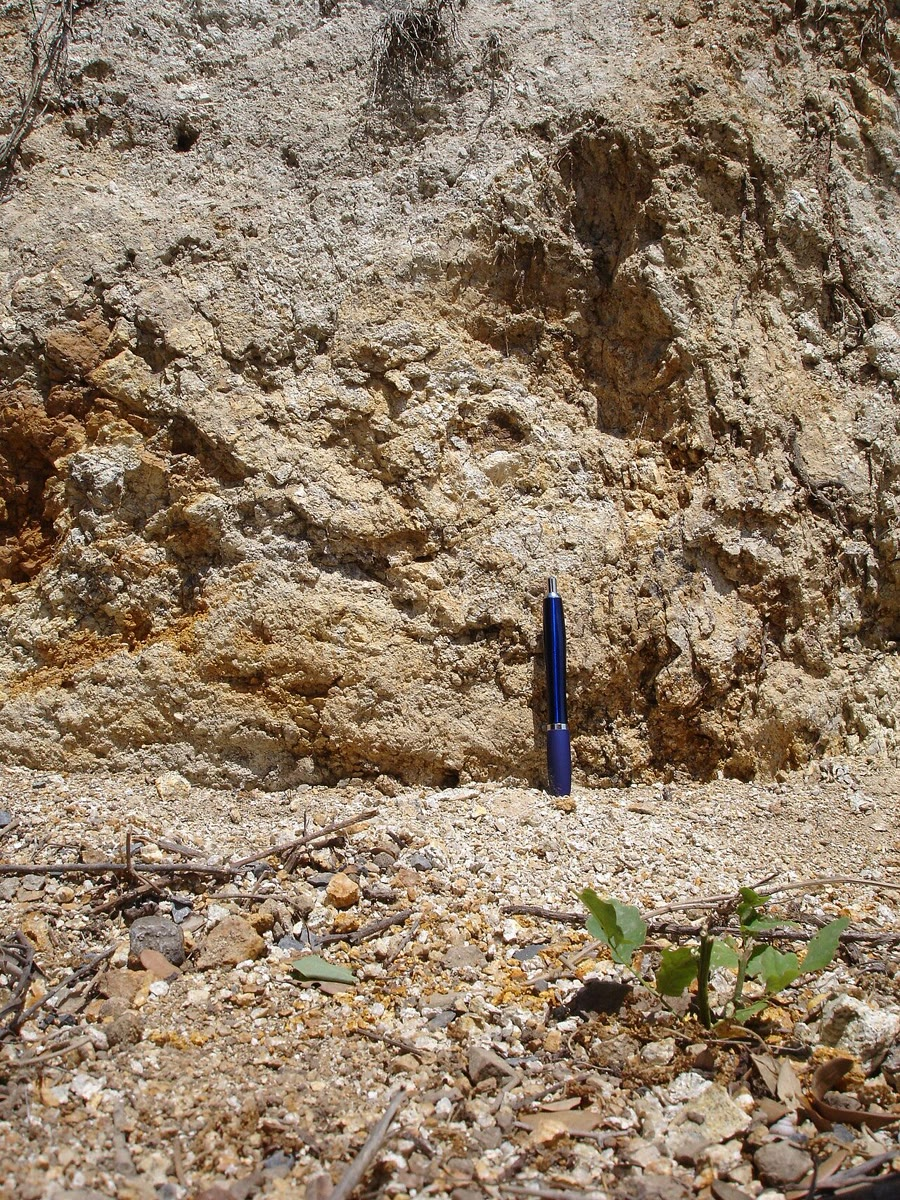
\includegraphics[height=6.3cm]{images/book3/b1-granite-grus.jpg}\hfill
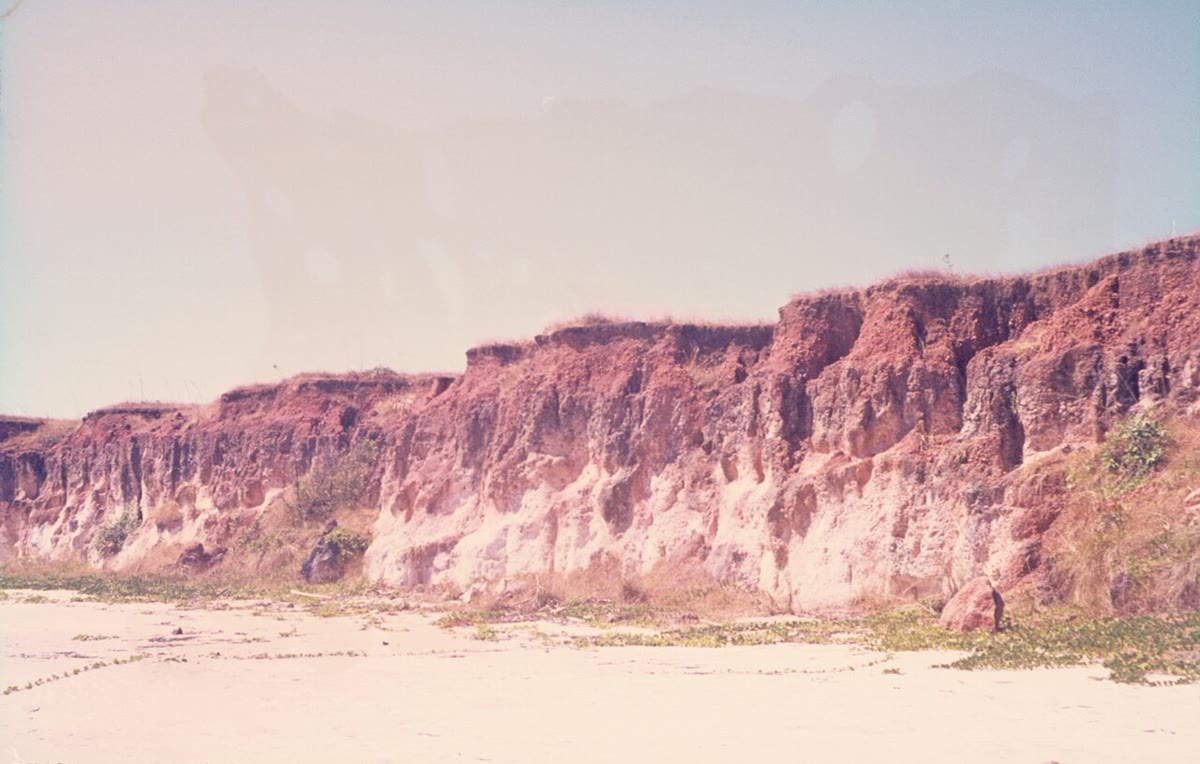
\includegraphics[height=6.3cm]{images/book3/b1-bauxite-weipa.jpg}
{\small À esquerda: granito podre nos Pirineus, ainda no lugar mas esfarelando-se em uma areia de quartzo, \omterm{def:b1:rock-forming-minerals:groups}{feldspato} e \omterm{def:b1:rock-forming-minerals:groups}{mica}, com a areia solta ao pé; a caneta dá a escala. Foto: Pinpin, CC~BY~2.5. À direita: um perfil de intemperismo na costa de Weipa, norte da Austrália: bauxita vermelha, produto da \omterm{def:b1:weathering-clays:hydrolysis-degree}{alitização}, sobre um arenito branco rico em \omterm{def:b1:weathering-clays:clay-mineral}{caulinita}. Foto: Werner Schellmann, 1969, CC~BY-SA~2.5. Ambas do Wikimedia Commons.}
\label{fig:b1:weathering-clays:photos}
\end{omfigure}
% ledger: commons:grus, commons:weipa

\emph{Quais \omterm{def:b1:rock-forming-minerals:mineral}{minerais} cedem primeiro.} Em 1938, Samuel Goldich, comparando perfis intemperizados com suas rochas-mãe, propôs uma série dos \omterm{def:b1:rock-forming-minerals:mineral}{minerais}, do menos ao mais estável no intemperismo, e constatou que ela segue a ordem em que cristalizam de um magma: \omterm{def:b1:rock-forming-minerals:groups}{olivina} e \omterm{def:b1:rock-forming-minerals:groups}{plagioclásio} rico em cálcio primeiro, quartzo por último. Os \omterm{def:b1:rock-forming-minerals:mineral}{minerais} formados nas temperaturas mais altas são os mais afastados do equilíbrio na superfície. Uma lista moderna, do menos ao mais resistente, diz: pirita, calcita, dolomita, \omterm{def:b1:rock-forming-minerals:groups}{olivina}, \omterm{def:b1:rock-forming-minerals:groups}{plagioclásio} cálcico, \omterm{def:b1:rock-forming-minerals:groups}{piroxênios}, \omterm{def:b1:rock-forming-minerals:groups}{plagioclásio} intermediário, \omterm{def:b1:rock-forming-minerals:groups}{anfibólios}, biotita, \omterm{def:b1:rock-forming-minerals:groups}{feldspato} potássico, muscovita, \omterm{def:b1:weathering-clays:clay-mineral}{esmectita}, quartzo, \omterm{def:b1:weathering-clays:clay-mineral}{caulinita}, e os óxidos gibbsita e hematita. Medidas de laboratório das taxas de dissolução confirmam a ordem; ela continua sendo uma ordem, não uma lei, pois a taxa de cada \omterm{def:b1:rock-forming-minerals:mineral}{mineral} depende também da água ao redor dele. Os produtos finais do intemperismo, \omterm{def:b1:weathering-clays:clay-mineral}{caulinita}, gibbsita e hematita, são os mais resistentes de todos: já são estáveis na superfície.
% ledger: goldich:1938, formoso:weatherability, lasaga:1984

\emph{O balanço de um perfil de intemperismo.} O intemperismo remove matéria, de modo que uma concentração medida em uma rocha intemperizada não diz quanto foi perdido: a perda de outros elementos concentra os que permanecem. Um elemento que não se move dá a referência.

\begin{proposition}[Balanço de massa com um elemento imóvel]\label{prop:b1:weathering-clays:immobile}
Seja $i$ um elemento que o intemperismo não move, com frações de massa $C_{i,p}$ na rocha-mãe e $C_{i,w}$ na rocha intemperizada. Então uma massa $m_p$ de rocha-mãe torna-se a massa $m_w = m_p C_{i,p}/C_{i,w}$ de rocha intemperizada, e a fração de qualquer outro elemento $j$ perdida é
\[
  f_j = 1 - \frac{C_{j,w}}{C_{j,p}}\,\frac{C_{i,p}}{C_{i,w}} .
\]
\end{proposition}

\begin{proof}
A massa de $i$ se conserva: $m_p C_{i,p} = m_w C_{i,w}$, o que dá $m_w$. A massa de $j$ passa de $m_p C_{j,p}$ a $m_w C_{j,w}$, uma fração
$m_w C_{j,w}/(m_p C_{j,p}) = (C_{j,w}/C_{j,p})(C_{i,p}/C_{i,w})$ dela permanece; $f_j$ é um menos essa fração.
\end{proof}

O titânio e o zircônio são as escolhas usuais, por uma razão que a próxima seção dá.

\section{Quais elementos saem: o potencial iônico}\label{sec:b1:weathering-clays:ionic}

Sódio, potássio e cálcio saem com a água; alumínio, ferro(III) e titânio permanecem; o silício está no meio. A diferença está no modo como cada íon se comporta na água.

\begin{definition}[Potencial iônico]\label{def:b1:weathering-clays:ionic-potential}
O \emph{potencial iônico}\index{potencial iônico} de um íon é a razão $z/r$ de seu número de carga $z$ ao seu raio iônico $r$, aqui em angströms (para a mesma coordenação para todos os íons, seis vezes, no que segue).
\end{definition}
% ledger: nomad:goldschmidt, dangic:goldschmidt, shannon:radii-b19

\begin{proposition}[Os três campos do potencial iônico]\label{prop:b1:weathering-clays:fields}
Na água do intemperismo, íons com $z/r < 3$ permanecem em solução como cátions hidratados e são levados embora (cátions solúveis); íons com $3 < z/r < 10$ ligam os íons hidróxido da água e precipitam como hidróxidos ou óxidos onde são liberados (hidrolisados); íons com $z/r > 10$ ligam o oxigênio com tanta força que repelem os íons hidrogênio e viajam como oxiânions solúveis, como carbonato, sulfato, fosfato e nitrato. O silício, com $z/r = 10$, está na fronteira, e é lixiviado em parte, mais quanto mais intenso o intemperismo.
\end{proposition}
\admitted
% ledger: nomad:goldschmidt, dangic:goldschmidt

A regra é empírica, devida a Victor Moritz Goldschmidt na década de 1930, e suas fronteiras são aproximadas; a química por trás dela, a atração entre um cátion e o oxigênio das moléculas de água ao seu redor, pertence aos livros de química. Um cátion pequeno e de carga alta puxa tão fortemente os elétrons de suas moléculas de água que elas perdem um íon hidrogênio e se tornam hidróxido: de modo moderado, e o hidróxido precipita; de modo extremo, e até o hidróxido perde seu hidrogênio, deixando um oxiânion.

O diagrama abaixo lê o intemperismo de uma rocha de relance. Sódio ($z/r = 0.98$), potássio (0.72), cálcio (2.0) e magnésio (2.8) saem: são os cátions da água de rios e do mar. Alumínio (5.6), ferro(III) (4.7), titânio (6.6) e zircônio (5.6) permanecem, e se acumulam nos perfis mais intemperizados; titânio e zircônio, que além disso estão em \omterm{def:b1:rock-forming-minerals:mineral}{minerais} que dificilmente se intemperizam, são as referências imóveis de \cref{prop:b1:weathering-clays:immobile}. O silício (10.0) é o elemento cuja perda parcial define os graus de \omterm{def:b1:weathering-clays:hydrolysis}{hidrólise}.
% ledger: shannon:radii-b19

A oxidação move um íon através da fronteira. O ferro(II), com $z/r = 2.6$, é um cátion solúvel; o ferro(III), com 4.7, um hidrolisado. Em um solo encharcado, sem oxigênio, o ferro se dissolve como \ce{Fe^2+} e é levado embora, deixando um solo cinzento; onde a água encontra o ar, em uma nascente ou em um solo bem drenado, o ferro é oxidado e precipita de imediato como óxidos vermelhos e marrons. O manganês se comporta do mesmo modo, \ce{Mn^2+} (2.4) contra \ce{Mn^4+} (7.5).
% ledger: nomad:goldschmidt, shannon:radii-b19

\begin{omfigure}
\begin{tikzpicture}[font=\small]
% ionic-potential diagram (figdata/bachelor-1/ionic_potential.py): charge against Shannon radius
\begin{axis}[width=12.5cm, height=8.4cm, xmin=0, xmax=1.8, ymin=0, ymax=7,
    xlabel={raio iônico $r$ (\si{\angstrom}, coordenação seis)}, ylabel={carga $z$},
    ytick={1,...,6}, xtick={0,0.2,...,1.8}, xticklabel style={/pgf/number format/fixed},
    axis on top, clip=true]
  \fill[omThm!14] (axis cs:0,0) -- (axis cs:1.8,0) -- (axis cs:1.8,5.4) -- cycle;
  \fill[omDef!16] (axis cs:0,0) -- (axis cs:1.8,5.4) -- (axis cs:1.8,7) -- (axis cs:0.7,7) -- cycle;
  \fill[omExo!18] (axis cs:0,0) -- (axis cs:0.7,7) -- (axis cs:0,7) -- cycle;
  \addplot[black, thick] table[x=r, y=z3] {figdata/out/bachelor-1-ionic_potential-lines.dat};
  \addplot[black, thick] table[x=r, y=z10] {figdata/out/bachelor-1-ionic_potential-lines.dat};
  \addplot[only marks, mark=*, mark size=1.6pt, black,
      point meta=explicit symbolic, nodes near coords,
      visualization depends on={value \thisrow{anc} \as \anc},
      every node near coord/.append style={font=\scriptsize, inner sep=2.6pt, anchor=\anc}]
    table[x=r, y=z, meta=tex] {figdata/out/bachelor-1-ionic_potential-ions.dat};
  \node[font=\footnotesize, align=center, fill=white, fill opacity=0.8, text opacity=1, rounded corners=1pt] at (axis cs:1.45,2.75) {cátions solúveis\\ $z/r < 3$};
  \node[font=\footnotesize, align=center, fill=white, fill opacity=0.8, text opacity=1, rounded corners=1pt] at (axis cs:1.15,6.3) {hidrolisados\\ $3 < z/r < 10$};
  \node[font=\footnotesize, align=left, fill=white, fill opacity=0.8, text opacity=1, rounded corners=1pt, anchor=north west] at (axis cs:0.015,6.95) {oxiânions solúveis, $z/r > 10$};
  \node[font=\scriptsize, rotate=28, anchor=south] at (axis cs:1.62,4.86) {$z/r = 3$};
  \node[font=\scriptsize, rotate=61, anchor=south] at (axis cs:0.2,2.0) {$z/r = 10$};
\end{axis}
\end{tikzpicture}

{\small O diagrama de \omterm{def:b1:weathering-clays:ionic-potential}{potencial iônico}: cada íon colocado por seu raio iônico efetivo em coordenação seis (Shannon, 1976) e sua carga. As retas $z/r = 3$ e $z/r = 10$ separam os íons que saem em solução como cátions, os que permanecem como hidróxidos ou óxidos, e os que saem como oxiânions. O silício jaz na fronteira superior.}
\label{fig:b1:weathering-clays:ionic-potential}
\end{omfigure}
% ledger: shannon:radii-b19, nomad:goldschmidt

\section{Argilominerais}\label{sec:b1:weathering-clays:clays}

\begin{definition}[Argilomineral, caulinita, ilita, esmectita, clorita]\label{def:b1:weathering-clays:clay-mineral}
Um \emph{argilomineral}\index{argilomineral} é um \omterm{def:b1:rock-forming-minerals:silicate-classes}{filossilicato} hidratado de alumínio, em geral em grãos de poucos micrômetros de diâmetro ou menos, formado por camadas que combinam uma lâmina tetraédrica (T) de tetraedros \ce{SiO4} que compartilham três vértices e uma lâmina octaédrica (O) de alumínio ou magnésio cercada por oxigênio e hidroxila. Na \emph{caulinita}\index{caulinita}, \ce{Al2Si2O5(OH)4}, cada camada é uma lâmina T e uma O (uma camada 1:1 ou T--O), sem carga, e as camadas são mantidas por ligações de hidrogênio. Nos argilominerais 2:1 ou T--O--T, uma lâmina O fica entre duas lâminas T voltadas para ela: a \emph{ilita}\index{ilita} é um argilomineral 2:1 não expansível, com íons potássio entre as camadas, como uma \omterm{def:b1:rock-forming-minerals:groups}{mica} com menos potássio; uma \emph{esmectita}\index{esmectita} é um argilomineral 2:1 com cátions hidratados e trocáveis e água entre suas camadas, que pode absorver mais água e inchar; uma \emph{clorita}\index{clorita} é um \omterm{def:b1:rock-forming-minerals:mineral}{mineral} 2:1 cujas camadas de carga negativa alternam com lâminas octaédricas de carga positiva do tipo da brucita, \ce{(Mg,Fe)(OH)2} com algum alumínio.
\end{definition}
% ledger: usgs:clay-groups, usgs:clay-settings, webmineral:clays-b19, biscaye:1965

A carga de uma camada decide como as camadas se empilham, e a carga vem de substituições nas lâminas (\cref{def:b1:rock-forming-minerals:substitution}).

\begin{proposition}[Carga de uma camada 2:1]\label{prop:b1:weathering-clays:layer-charge}
Uma camada 2:1 de fórmula $\mathrm{(Si_{4-x}Al_x)(Al_{2-y}Mg_y)O_{10}(OH)_2}$, com $x$ alumínios no lugar de silício em suas lâminas tetraédricas e $y$ magnésios no lugar de alumínio em sua lâmina octaédrica, tem a carga $-(x + y)$ por unidade de fórmula.
\end{proposition}

\begin{proof}
Some as cargas: $4(4 - x) + 3x$ dos cátions tetraédricos, $3(2 - y) + 2y$ dos octaédricos, $-2\times10$ dos oxigênios e $-1\times2$ das hidroxilas: $16 - x + 6 - y - 20 - 2 = -(x + y)$.
\end{proof}

Sem substituição ($x = y = 0$) a camada é neutra, como em \ce{Al2Si4O10(OH)2}, o \omterm{def:b1:rock-forming-minerals:mineral}{mineral} pirofilita, e as camadas são mantidas apenas por forças fracas. Na moscovita, $x = 1$, uma carga de $-1$ é balanceada por um íon potássio que trava as camadas juntas; a \omterm{def:b1:weathering-clays:clay-mineral}{ilita} fica perto dela, com um pouco menos. Na beidelita de \cref{prop:b1:weathering-clays:feldspars}, $x = 0.5$: a carga $-0.5$ é balanceada por $0.5$ sódio. Uma carga menor mantém as camadas menos firmemente presas, e entre elas podem entrar água e cátions hidratados: é por isso que as \omterm{def:b1:weathering-clays:clay-mineral}{esmectitas}, com cargas de cerca de 0.3 a 0.5 por unidade de fórmula, como nas fórmulas da montmorilonita e da beidelita, incham, enquanto a \omterm{def:b1:weathering-clays:clay-mineral}{ilita} não. Os cátions entre as camadas de uma \omterm{def:b1:weathering-clays:clay-mineral}{esmectita} são trocáveis, e a capacidade de troca dos argilominerais comuns segue sua estrutura: de 3 a 15 miliequivalentes por \qty{100}{g} para a \omterm{def:b1:weathering-clays:clay-mineral}{caulinita}, cujas camadas não têm carga, de 10 a 40 para a \omterm{def:b1:weathering-clays:clay-mineral}{ilita}, de 70 a 100 para a montmorilonita, uma \omterm{def:b1:weathering-clays:clay-mineral}{esmectita}. O potássio, que trava as camadas de uma \omterm{def:b1:rock-forming-minerals:groups}{mica}, favorece a \omterm{def:b1:weathering-clays:clay-mineral}{ilita}; as \omterm{def:b1:weathering-clays:clay-mineral}{esmectitas} se formam onde o potássio é escasso e cálcio e magnésio estão disponíveis.
% ledger: webmineral:clays-b19, carroll:cec, usgs:clay-settings

\begin{omfigure}
\begin{tikzpicture}[font=\footnotesize, >={Stealth[length=4pt]}, y=0.2cm, x=1cm]
% schematic clay-mineral structures, vertical scale proportional to the basal spacings
% (USGS OFR 01-041, ledger usgs:clay-xrd): kaolinite 7, illite 10, smectite 14 (air-dried), chlorite 14 angstrom.
% T sheet 2 A thick, O sheet 2.4 A thick (schematic); the column width is 2.2 cm.
\def\W{2.2}
\newcommand{\Tsheet}[1]{% tetrahedral sheet whose base is at y=#1
  \fill[omDef!35] (0,#1) rectangle (\W,#1+2);
  \foreach \i in {0,...,6} {\draw[omDef!80!black, line width=0.4pt] (0.04+\i*0.31,#1) -- (0.195+\i*0.31,#1+2) -- (0.35+\i*0.31,#1) -- cycle;}
}
\newcommand{\TsheetDown}[1]{% inverted tetrahedral sheet, base at the top (y=#1+2)
  \fill[omDef!35] (0,#1) rectangle (\W,#1+2);
  \foreach \i in {0,...,6} {\draw[omDef!80!black, line width=0.4pt] (0.04+\i*0.31,#1+2) -- (0.195+\i*0.31,#1) -- (0.35+\i*0.31,#1+2) -- cycle;}
}
\newcommand{\Osheet}[2]{% octahedral sheet, base at y=#1, fill colour #2
  \fill[#2] (0,#1) rectangle (\W,#1+2.4);
  \foreach \i in {0,...,4} {\draw[black!55, line width=0.4pt] (0.17+\i*0.42,#1+1.2) -- ++(0.17,1.0) -- ++(0.17,-1.0) -- ++(-0.17,-1.0) -- cycle;}
}
\newcommand{\spacing}[3]{% arrow for d001 from y=#1 to y=#2 with label #3
  \draw[<->, line width=0.5pt] (\W+0.18,#1) -- (\W+0.18,#2) node[midway, right, inner sep=2pt] {#3};
  \draw[black!40, densely dotted] (\W,#1) -- (\W+0.28,#1); \draw[black!40, densely dotted] (\W,#2) -- (\W+0.28,#2);
}
% ---------- kaolinite: T-O, d = 7.2
\begin{scope}[xshift=0cm]
  \foreach \b in {0, 7.2} {\Tsheet{\b} \Osheet{\b+2}{omThm!25}}
  \spacing{0}{7.2}{\SI{7}{\angstrom}}
  \node[anchor=north, align=center] at (\W/2,-0.8) {\textbf{caulinita}\\ camadas T--O (1:1)\\ mantidas por ligações de hidrogênio};
\end{scope}
% ---------- illite: T-O-T + K, d = 10
\begin{scope}[xshift=3.6cm]
  \foreach \b in {0, 10} {\Tsheet{\b} \Osheet{\b+2}{omThm!25} \TsheetDown{\b+4.4}}
  \foreach \b in {6.4} {\foreach \i in {0,...,4} \fill[omExo!70!black] (0.25+\i*0.42,\b+1.8) circle[radius=1.5pt];}
  \spacing{0}{10}{\SI{10}{\angstrom}}
  \node[anchor=north, align=center] at (\W/2,-0.8) {\textbf{ilita}\\ camadas T--O--T (2:1)\\ mantidas por íons \ce{K+}};
\end{scope}
% ---------- smectite: T-O-T + hydrated cations, d = 14
\begin{scope}[xshift=7.2cm]
  \foreach \b in {0, 14} {\Tsheet{\b} \Osheet{\b+2}{omThm!25} \TsheetDown{\b+4.4}}
  \foreach \i in {0,...,9} {\draw[omDef!60, line width=0.3pt] (0.13+\i*0.215,8.6) circle[radius=1.3pt]; \draw[omDef!60, line width=0.3pt] (0.2+\i*0.215,11.8) circle[radius=1.3pt];}
  \foreach \i in {0,...,3} {\fill[omExo!70!black] (0.35+\i*0.5,10.2) circle[radius=1.5pt];}
  \spacing{0}{14}{\SI{14}{\angstrom}}
  \node[anchor=north, align=center] at (\W/2,-0.8) {\textbf{esmectita}\\ camadas T--O--T, hidratadas\\ \ce{Na+}, \ce{Ca^2+} e água};
\end{scope}
% ---------- chlorite: T-O-T + brucite-like O sheet, d = 14
\begin{scope}[xshift=10.8cm]
  \foreach \b in {0, 14} {\Tsheet{\b} \Osheet{\b+2}{omThm!25} \TsheetDown{\b+4.4}}
  \Osheet{9}{omExo!25}
  \spacing{0}{14}{\SI{14}{\angstrom}}
  \node[anchor=north, align=center] at (\W/2,-0.8) {\textbf{clorita}\\ camadas T--O--T e uma\\ lâmina O tipo brucita};
\end{scope}
% key
\begin{scope}[xshift=0cm, yshift=-2.75cm]
  \fill[omDef!35] (0,0) rectangle (0.4,1.6); \draw[omDef!80!black] (0.05,0) -- (0.2,1.6) -- (0.35,0) -- cycle;
  \node[anchor=west] at (0.5,0.8) {T: lâmina tetraédrica, \ce{SiO4} (alguns \ce{AlO4})};
  \fill[omExo!70!black] (8.1,0.8) circle[radius=1.5pt]; \node[anchor=west] at (8.3,0.8) {cátion entre as camadas};
  \fill[omThm!25] (0,-2.6) rectangle (0.4,-1.0);
  \node[anchor=west] at (0.5,-1.8) {O: lâmina octaédrica, \ce{Al} ou \ce{Mg} com \ce{O} e \ce{OH}};
  \draw[omDef!60] (8.1,-1.8) circle[radius=1.3pt]; \node[anchor=west] at (8.3,-1.8) {molécula de água};
\end{scope}
\end{tikzpicture}

{\small As quatro famílias de argilominerais (esquemático, duas camadas de cada). A escala vertical é proporcional ao espaçamento basal, a distância de repetição de uma camada para a seguinte medida por difração de raios X: \SI{7}{\angstrom} para \omterm{def:b1:weathering-clays:clay-mineral}{caulinita}, \SI{10}{\angstrom} para \omterm{def:b1:weathering-clays:clay-mineral}{ilita}, cerca de \SI{14}{\angstrom} para uma \omterm{def:b1:weathering-clays:clay-mineral}{esmectita} seca ao ar e para a \omterm{def:b1:weathering-clays:clay-mineral}{clorita}.}
\label{fig:b1:weathering-clays:structures}
\end{omfigure}
% ledger: usgs:clay-xrd, usgs:clay-groups



\begin{table}[htbp]
\centering\footnotesize
\setlength{\tabcolsep}{4pt}
% ledger: usgs:clay-xrd, usgs:clay-groups, usgs:clay-settings, carroll:cec, biscaye:1965
\begin{tabular}{@{}>{\raggedright\arraybackslash}p{1.6cm}>{\raggedright\arraybackslash}p{1.5cm}>{\raggedright\arraybackslash}p{1.6cm}>{\raggedright\arraybackslash}p{1.5cm}>{\raggedright\arraybackslash}p{1.4cm}>{\raggedright\arraybackslash}p{1.4cm}>{\raggedright\arraybackslash}p{1.2cm}>{\raggedright\arraybackslash}p{3.2cm}@{}}
\hline
\omterm{def:b1:rock-forming-minerals:mineral}{mineral} & camada & entre camadas & seco ao ar & glicol & aquecido & CTC & ambiente típico \\
\hline
\omterm{def:b1:weathering-clays:clay-mineral}{caulinita} & T--O & nenhum & \SI{7}{\angstrom} & \SI{7}{\angstrom} & destruída a \SI{550}{\celsius} & 3--15 & \omterm{def:b1:rock-forming-minerals:groups}{feldspatos} lixiviados por água ácida; intemperismo tropical intenso \\
\omterm{def:b1:weathering-clays:clay-mineral}{ilita} & T--O--T & \ce{K+} & \SI{10}{\angstrom} & \SI{10}{\angstrom} & \SI{10}{\angstrom} & 10--40 & água alcalina rica em K; a partir de \omterm{def:b1:rock-forming-minerals:groups}{feldspatos} e \omterm{def:b1:rock-forming-minerals:groups}{micas}; a argila principal dos lamitos \\
\omterm{def:b1:weathering-clays:clay-mineral}{esmectita} & T--O--T & \ce{Na+}, \ce{Ca^2+} hidratados & cerca de \SI{14}{\angstrom} & \SI{17}{\angstrom} & \SI{10}{\angstrom} a \SI{400}{\celsius} & 70--100 & rochas básicas intemperizadas; terreno mal drenado, K escasso \\
\omterm{def:b1:weathering-clays:clay-mineral}{clorita} & T--O--T & lâmina tipo brucita & \SI{14}{\angstrom} & \SI{14}{\angstrom} & \SI{14}{\angstrom} & -- & rochas metamórficas de baixo grau e ígneas alteradas; lamitos \\
\hline
\end{tabular}
\caption{As quatro famílias de argilominerais: estrutura, espaçamento basal medido em lâminas orientadas secas ao ar, após solvatação com etilenoglicol e após aquecimento, capacidade de troca de cátions (CTC, miliequivalentes por \qty{100}{g}; o valor da \omterm{def:b1:weathering-clays:clay-mineral}{esmectita} é o da montmorilonita) e onde costumam se formar.}
\label{tab:b1:weathering-clays:clays}
\end{table}

\begin{inthelab}[Identificando argilominerais por difração de raios X]
Argilominerais são finos demais para serem distinguidos ao microscópio óptico. No laboratório, a fração mais fina de um solo ou de um lamito é separada deixando os grãos mais grossos sedimentarem na água, e uma gota da suspensão é seca sobre uma lâmina de vidro, onde as lâminas jazem planas: uma lâmina orientada. Os raios X refletidos pelas camadas empilhadas dão picos fortes nos ângulos fixados pelo espaçamento basal, pela lei de Bragg da difração (física). A lâmina é passada três ou quatro vezes: seca ao ar; após uma noite em vapor de etilenoglicol, que entra entre as camadas das \omterm{def:b1:weathering-clays:clay-mineral}{esmectitas} e as incha até \SI{17}{\angstrom}, deixando os outros \omterm{def:b1:rock-forming-minerals:mineral}{minerais} inalterados; após aquecimento a \SI{400}{\celsius}, que expele a água das \omterm{def:b1:weathering-clays:clay-mineral}{esmectitas} e as colapsa para \SI{10}{\angstrom}; e após aquecimento a \SI{550}{\celsius}, que destrói a \omterm{def:b1:weathering-clays:clay-mineral}{caulinita} mas deixa a \omterm{def:b1:weathering-clays:clay-mineral}{ilita} e a \omterm{def:b1:weathering-clays:clay-mineral}{clorita}. \Cref{tab:b1:weathering-clays:clays} é a chave para ler as quatro medidas; misturas e \omterm{def:b1:rock-forming-minerals:mineral}{minerais} interestratificados, muito comuns em solos, exigem mais.
\end{inthelab}
% ledger: usgs:clay-xrd

\begin{omfigure}
\begin{minipage}[t]{0.66\linewidth}\vspace{0pt}
\emph{Argilas como indicadores de clima.} Como o grau da \omterm{def:b1:weathering-clays:hydrolysis}{hidrólise} segue o clima, os argilominerais de um solo o registram: \omterm{def:b1:weathering-clays:clay-mineral}{caulinita} e gibbsita onde o intemperismo é intenso, sob climas quentes e úmidos; \omterm{def:b1:weathering-clays:clay-mineral}{esmectitas} onde a água é pouco renovada; onde o intemperismo é fraco, as argilas são sobretudo herdadas da rocha, \omterm{def:b1:weathering-clays:clay-mineral}{ilita} e \omterm{def:b1:weathering-clays:clay-mineral}{clorita} de \omterm{def:b1:rock-forming-minerals:groups}{micas} e xistos. Os rios levam essas argilas ao mar, e as lamas do fundo oceânico guardam o registro: ao largo dos pequenos rios da América do Sul tropical, ricos em \omterm{def:b1:weathering-clays:clay-mineral}{caulinita} e gibbsita, elas mostram o intemperismo intenso da terra que drenam. Quando solos são soterrados e preservados, seus argilominerais servem para inferir os climas do passado geológico: um leito rico em \omterm{def:b1:weathering-clays:clay-mineral}{caulinita} numa sequência de lamitos ricos em \omterm{def:b1:weathering-clays:clay-mineral}{ilita} aponta para um episódio quente e úmido. Tal inferência exige cuidado, pois os argilominerais também são transportados para longe de onde se formaram, e se transformam com o soterramento, as \omterm{def:b1:weathering-clays:clay-mineral}{esmectitas} se tornando \omterm{def:b1:weathering-clays:clay-mineral}{ilita} à medida que são aquecidas (\cref{ch:b1:diagenesis-basins}).
\end{minipage}\hfill
\begin{minipage}[t]{0.30\linewidth}\vspace{0pt}
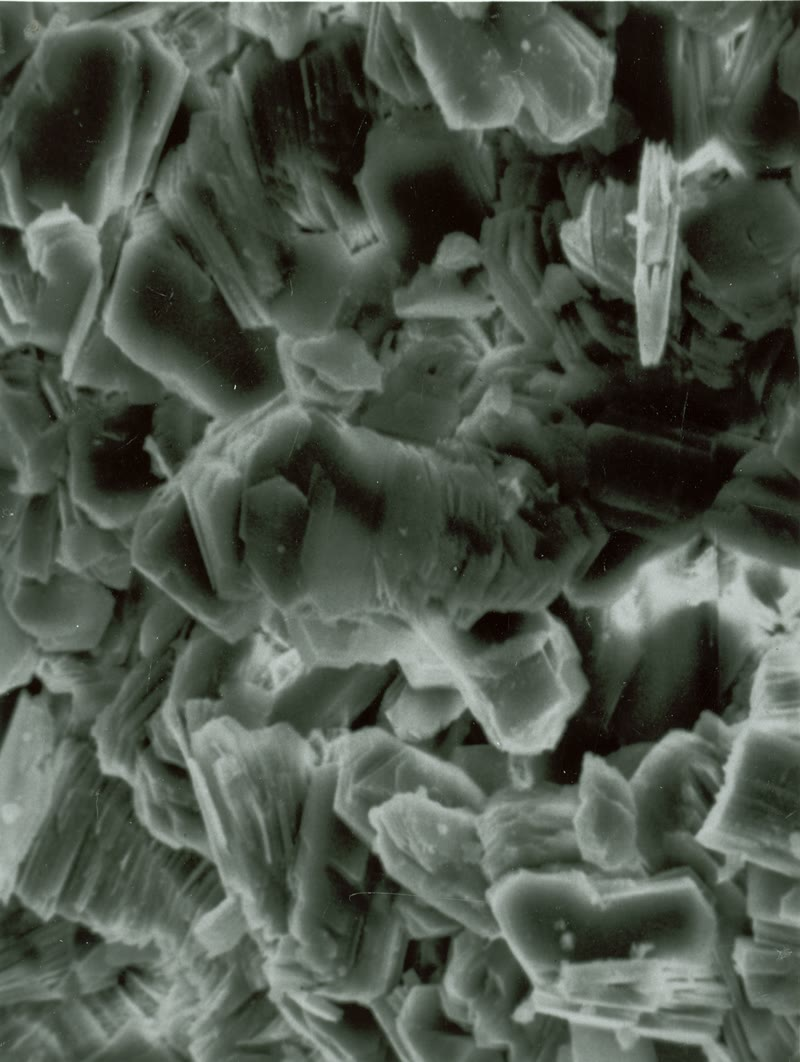
\includegraphics[width=\linewidth]{images/book3/b1-kaolinite-sem.jpg}

{\scriptsize \omterm{def:b1:weathering-clays:clay-mineral}{Caulinita} vista ao microscópio eletrônico de varredura: livros de placas hexagonais empilhadas crescidos nos poros de um arenito do norte do Alasca (ampliação de cerca de 1340). Serviço Geológico dos Estados Unidos, domínio público, via Wikimedia Commons.\par}
\end{minipage}
\end{omfigure}
% ledger: biscaye:1965, usgs:clay-settings, pedron:stages, commons:kaolinite-sem

\emph{\omterm{def:b1:weathering-clays:laterite}{Lateritas}.} Onde a \omterm{def:b1:weathering-clays:hydrolysis}{hidrólise} atinge seus últimos graus por muito tempo, o perfil se espessa, e seu topo concentra tudo o que não sai.

\begin{definition}[Laterita]\label{def:b1:weathering-clays:laterite}
Uma \emph{laterita}\index{laterita} é o produto rico em ferro e alumínio de \omterm{def:b1:weathering-clays:hydrolysis}{hidrólise} intensa e prolongada sob climas quentes e úmidos: um material vermelho a marrom, mole ou endurecido, formado por \omterm{def:b1:weathering-clays:clay-mineral}{caulinita} e óxidos e hidróxidos de ferro, com gibbsita onde a \omterm{def:b1:weathering-clays:hydrolysis-degree}{alitização} é atingida, do qual quase todos os cátions alcalinos e alcalino-terrosos e grande parte da sílica foram removidos.
\end{definition}
% ledger: formoso:laterite, buchanan:laterite

Uma \omterm{def:b1:weathering-clays:laterite}{laterita} rica o bastante em gibbsita ou boehmita, os hidróxidos de alumínio, é uma bauxita, o minério de quase nove décimos do alumínio: a \omterm{def:b1:weathering-clays:hydrolysis-degree}{alitização} é a etapa que faz o minério. A maioria das bauxitas é residual, a rocha da qual tudo, exceto a alumina, foi lixiviado; a maioria das formadas por gibbsita jaz nos trópicos, e muitas provavelmente ainda se formam.
% ledger: usgs:bauxite

\begin{history}[Uma palavra do campo]
Em 1807, Francis Buchanan, viajando em Malabar, no sul da Índia, descreveu um material cheio de cavidades e rico em ocres vermelhos e amarelos de ferro, espalhado sobre o granito em grandes massas. Extraído do solo, era tão mole que uma faca o cortava, e os habitantes o moldavam em blocos; no ar logo se tornava tão duro quanto tijolo, e durava melhor que qualquer tijolo que ele tivesse visto. As línguas locais o chamavam de pedra-tijolo; ele propôs o nome \omterm{def:b1:weathering-clays:laterite}{laterita}, que a geologia guardou para os produtos vermelhos do intemperismo tropical.
\end{history}
% ledger: buchanan:laterite

\section{Intemperismo de silicatos e gás carbônico}\label{sec:b1:weathering-clays:co2}

Os íons hidrogênio da \omterm{def:b1:weathering-clays:hydrolysis}{hidrólise} vêm sobretudo do gás carbônico, então escrevê-los como ácido carbônico mostra o que o intemperismo faz ao ar. Para um silicato de cálcio, escrito \ce{CaSiO3} por simplicidade,
\[
  \ce{CaSiO3 + 2 CO2 + H2O -> Ca^2+ + 2 HCO3- + SiO2},
\]
e no oceano, onde os organismos constroem conchas de carbonato de cálcio,
\[
  \ce{Ca^2+ + 2 HCO3- -> CaCO3 + CO2 + H2O}.
\]

\begin{proposition}[Intemperismo e gás carbônico]\label{prop:b1:weathering-clays:co2}
(a) O intemperismo de um silicato consome dois moles de gás carbônico, transformados em bicarbonato, para cada mol de cálcio ou magnésio liberado; quando o cálcio ou o magnésio são precipitados como carbonato, um dos dois retorna ao ar, e um mol fica armazenado como rocha carbonática. (b) O intemperismo de uma rocha carbonática e a precipitação de seu carbonato de novo não armazenam nenhum.
\end{proposition}

\begin{proof}
(a) Somando as duas equações acima dá \ce{CaSiO3 + CO2 -> CaCO3 + SiO2}: um \ce{CO2} por cálcio sai do ar para sempre; a primeira equação sozinha mostra os dois consumidos. Para o magnésio vale o mesmo, com \ce{Mg^2+} no lugar de
\ce{Ca^2+}. (b) A dissolução da calcita, \ce{CaCO3 + CO2 + H2O -> Ca^2+ + 2
HCO3-}, é exatamente o inverso da precipitação: a soma das duas é zero.
\end{proof}

Com um \omterm{def:b1:rock-forming-minerals:groups}{feldspato}, o ácido carbônico substitui os íons hidrogênio de \cref{prop:b1:weathering-clays:feldspars}: cada \ce{H+} consumido é um \ce{CO2} transformado em \ce{HCO3-}. A anortita de um basalto ou de um gabro consome, assim, dois moles de gás carbônico por mol ao se transformar em \omterm{def:b1:weathering-clays:clay-mineral}{caulinita},
\[
  \ce{CaAl2Si2O8 + 2 CO2 + 3 H2O -> Al2Si2O5(OH)4 + Ca^2+ + 2 HCO3-},
\]
e armazena um no longo prazo. Sódio e potássio não formam carbonato no fundo do mar, e o armazenamento de longo prazo é contado a partir do cálcio e do magnésio liberados.

Os rios levam o bicarbonato ao mar, e sua química mede o fluxo. A partir da química dos grandes rios do mundo, o gás carbônico consumido pelo intemperismo de silicatos continentais foi estimado em \num{11.7e12} a \qty{13.6e12}{mol} por ano, cerca de 0.14 a 0.16 bilhão de toneladas de carbono, das quais o intemperismo dos basaltos sozinho responde por 30 a \qty{35}{\percent}. O fluxo é pequeno diante das trocas de carbono entre o ar, os oceanos e os seres vivos, mas não se inverte: ao longo de milhões de anos é o principal modo pelo qual o gás carbônico fornecido por vulcões sai da atmosfera. Como o intemperismo corre mais depressa quando é mais quente e mais úmido, ele liga o gás carbônico do ar ao clima, que por sua vez depende do gás carbônico pelo efeito estufa: uma retroalimentação negativa que estabiliza a temperatura da Terra ao longo do tempo geológico, estudada no volume do Livro 4.
% ledger: dessert:silicate-co2, whk:1981

\section{Exercícios}

\begin{exercise}[$\star$]\label{exo:b1:weathering-clays:1}
Usando os raios \ce{K+} \qty{1.38}{\angstrom}, \ce{Fe^2+} \qty{0.78}{\angstrom},
\ce{Fe^3+} \qty{0.645}{\angstrom} e \ce{Ti^4+} \qty{0.605}{\angstrom}, calcule o \omterm{def:b1:weathering-clays:ionic-potential}{potencial iônico} de cada íon e dê o nome de seu campo. Por que um solo encharcado perde seu ferro enquanto um bem drenado o conserva?
% ledger: shannon:radii-b19
\end{exercise}

\begin{exercise}[$\star$]\label{exo:b1:weathering-clays:2}
Quatro frações de argila são analisadas por raios X como lâminas orientadas. A: um pico em
\SI{14}{\angstrom}, deslocado para \SI{17}{\angstrom} pelo etilenoglicol e para \SI{10}{\angstrom} por aquecimento a \SI{400}{\celsius}. B: um pico em \SI{7}{\angstrom}, inalterado pelo glicol, desaparecido após aquecimento a
\SI{550}{\celsius}. C: um pico em \SI{10}{\angstrom} que nenhum tratamento desloca. D: um pico em \SI{14}{\angstrom} que nenhum tratamento desloca. Identifique cada \omterm{def:b1:rock-forming-minerals:mineral}{mineral}.
% ledger: usgs:clay-xrd
\end{exercise}

\begin{exercise}[$\star$]\label{exo:b1:weathering-clays:3}
Balanceie, com \cref{met:b1:weathering-clays:balance}, a \omterm{def:b1:weathering-clays:hydrolysis}{hidrólise} do ortoclásio
\ce{KAlSi3O8} em \omterm{def:b1:weathering-clays:clay-mineral}{caulinita}. Que fração de seu potássio e de seu silício sai em solução?
\end{exercise}

\begin{exercise}[$\star$]\label{exo:b1:weathering-clays:4}
(a) Que volume de gelo dá \qty{10}{cm^3} de água a \qty{0}{\celsius}? (b) Dentro de que faixa de temperatura o gelo que cresce em fissuras racha a rocha de modo mais eficaz, e por que nem uma geada mais leve nem uma mais dura fazem tão bem? (c) Um cubo de granito de lado \qty{1}{m} é fragmentado pela geada em cubos de lado \qty{1}{cm}: por que fator sua área de superfície cresceu?
% ledger: usgs:water-density, iapws:ice-density, wh85:frost
\end{exercise}

\begin{exercise}[$\star\star$]\label{exo:b1:weathering-clays:5}
Calcule a superfície específica de grãos de \omterm{def:b1:rock-forming-minerals:groups}{feldspato} de densidade
\qty{2600}{kg.m^{-3}}, tratados como cubos, para tamanhos de \qty{1}{cm}, \qty{1}{mm} e \qty{1}{\micro m}. Por que o tamanho do grão importa tanto para a taxa do \omterm{def:b1:weathering-clays:weathering}{intemperismo químico}, e por que o \omterm{def:b1:weathering-clays:weathering}{intemperismo físico} acelera o químico?
\end{exercise}

\begin{exercise}[$\star\star$]\label{exo:b1:weathering-clays:6}
Uma tonelada de albita \ce{NaAlSi3O8} (\qty{262.22}{g.mol^{-1}}) transforma-se em \omterm{def:b1:weathering-clays:clay-mineral}{caulinita} (\qty{258.16}{g.mol^{-1}}). Calcule a massa de \omterm{def:b1:weathering-clays:clay-mineral}{caulinita} formada, a massa de sílica exportada, contada como \ce{SiO2} (\qty{60.08}{g.mol^{-1}}), e a massa de sódio exportada.
% ledger: webmineral:clays-b19, ciaaw:Na
\end{exercise}

\begin{exercise}[$\star\star$]\label{exo:b1:weathering-clays:7}
Um granito contém, em massa, \qty{0.30}{\percent} \ce{TiO2}, \qty{3.5}{\percent}
\ce{Na2O}, \qty{72}{\percent} \ce{SiO2} e \qty{14}{\percent} \ce{Al2O3}; seu saprólito contém \qty{0.60}{\percent} \ce{TiO2}, \qty{0.35}{\percent}
\ce{Na2O}, \qty{60}{\percent} \ce{SiO2} e \qty{27}{\percent} \ce{Al2O3}. Tomando o titânio como imóvel, encontre a massa de saprólito deixada por um quilograma de granito e a fração de sódio, silício e alumínio perdida. Qual grau de \omterm{def:b1:weathering-clays:hydrolysis}{hidrólise} está em curso?
\end{exercise}

\begin{exercise}[$\star\star$]\label{exo:b1:weathering-clays:8}
Usando \cref{prop:b1:weathering-clays:layer-charge}, calcule a carga da camada da pirofilita \ce{Al2Si4O10(OH)2}, da moscovita \ce{KAl2(Si3Al)O10(OH)2} sem seu potássio, da camada de beidelita \ce{Al2(Si_{3.5}Al_{0.5})O10(OH)2} e de uma camada de montmorilonita \ce{(Al_{1.67}Mg_{0.33})Si4O10(OH)2}. Qual deles pode inchar, e por quê?
% ledger: webmineral:clays-b19
\end{exercise}

\begin{exercise}[$\star\star$]\label{exo:b1:weathering-clays:9}
Forsterita \ce{Mg2SiO4} se intemperiza por
\ce{Mg2SiO4 + 4 CO2 + 4 H2O -> 2 Mg^2+ + 4 HCO3- + H4SiO4}. (a) Confira a equação. (b) Para uma tonelada de forsterita, calcule o gás carbônico consumido e o gás carbônico armazenado a longo prazo segundo a
\cref{prop:b1:weathering-clays:co2}. (c) O que daria o mesmo cálculo para uma tonelada de calcita?
% ledger: ciaaw:Mg, ciaaw:Si, ciaaw:O, ciaaw:C
\end{exercise}

\begin{exercise}[$\star\star\star$]\label{exo:b1:weathering-clays:10}
(a) Entre quais raios um íon de carga 3 é um hidrolisado? (b) O boro, \ce{B^3+}, tem raio de \qty{0.27}{\angstrom}: em que forma ele viaja na água? (c) \ce{Mn^2+} tem raio de \qty{0.83}{\angstrom}, \ce{Mn^4+} de \qty{0.53}{\angstrom}. Explique por que \omterm{def:b1:layered-earth:layers}{crostas} pretas de óxido de manganês se formam onde a água de nascente, pobre em oxigênio, aflora ao ar. (d) Por que o silício pode ser nem totalmente lixiviado nem totalmente retido?
% ledger: shannon:radii-b19, nomad:goldschmidt
\end{exercise}

\begin{exercise}[$\star\star\star$]\label{exo:b1:weathering-clays:11}
O intemperismo dos silicatos continentais consome \num{11.7e12} a
\qty{13.6e12}{mol} de gás carbônico por ano, \qty{4.08e12}{mol} dele dos basaltos. (a) Converta a faixa em toneladas de carbono e de gás carbônico por ano. (b) Que parcela tomam os basaltos? (c) Se tudo isso viesse de silicatos de cálcio e magnésio, quanto carbono seria armazenado a longo prazo a cada ano? Por que o valor real de longo prazo é menor?
% ledger: dessert:silicate-co2, ciaaw:C, ciaaw:O
\end{exercise}

\begin{exercise}[$\star\star\star$]\label{exo:b1:weathering-clays:12}
Três frações de argila, livres de quartzo e de óxidos de ferro, são analisadas (porcentagem em massa): A, \ce{SiO2} \num{46.55} e \ce{Al2O3} \num{39.50}; B, \ce{SiO2} 60 e
\ce{Al2O3} 25; C, \ce{SiO2} 2 e \ce{Al2O3} 63 (\ce{SiO2}
\qty{60.08}{g.mol^{-1}}, \ce{Al2O3} \qty{101.96}{g.mol^{-1}}). Calcule a razão molar Si/Al de cada uma, identifique o grau de \omterm{def:b1:weathering-clays:hydrolysis}{hidrólise} que ela registra, e coloque as três argilas numa linha, da lixiviação menos à mais intensa.
% ledger: webmineral:clays-b19, pedron:stages, formoso:laterite
\end{exercise}

\section{Problema: do granito à argila}

\begin{problem}[{Problema de fim de semana --- os feldspatos de um granito e de um gabro, das reações balanceadas ao gás carbônico que um rio carrega}]
\label{pb:b1:weathering-clays:1}
% values: calc/ch19.py; the river is invented (its numbers are of a realistic order)
Os \omterm{def:b1:rock-forming-minerals:groups}{feldspatos} são a albita \ce{NaAlSi3O8} (\qty{262.22}{g.mol^{-1}}, densidade
\qty{2.62}{g.cm^{-3}}) e a anortita \ce{CaAl2Si2O8}
(\qty{278.20}{g.mol^{-1}}, densidade \qty{2.75}{g.cm^{-3}}). A \omterm{def:b1:weathering-clays:clay-mineral}{caulinita}
\ce{Al2Si2O5(OH)4} tem massa molar \qty{258.16}{g.mol^{-1}} e densidade
\qty{2.6}{g.cm^{-3}}; a gibbsita \ce{Al(OH)3}, \qty{78.00}{g.mol^{-1}}. Tome
\ce{SiO2} \qty{60.08}{g.mol^{-1}}, \ce{CO2} \qty{44.01}{g.mol^{-1}}, \ce{HCO3-}
\qty{61.02}{g.mol^{-1}}, Na \num{22.99} e Ca \qty{40.08}{g.mol^{-1}}.
% ledger: hom:albite, hom:anorthite, webmineral:clays-b19, ciaaw:Na, ciaaw:Ca, ciaaw:C, ciaaw:O, ciaaw:H

\medskip
\noindent\textbf{Parte I --- As reações.}
\begin{enumerate}
  \item Balanceie a \omterm{def:b1:weathering-clays:hydrolysis}{hidrólise} da albita em \omterm{def:b1:weathering-clays:clay-mineral}{caulinita}.
  \item Balanceie a \omterm{def:b1:weathering-clays:hydrolysis}{hidrólise} da anortita em \omterm{def:b1:weathering-clays:clay-mineral}{caulinita}. O que há de especial nela?
  \item Balanceie a \omterm{def:b1:weathering-clays:hydrolysis}{hidrólise} da anortita em gibbsita.
  \item Balanceie a \omterm{def:b1:weathering-clays:hydrolysis}{hidrólise} da albita em beidelita
        \ce{Na_{0.5}Al2(Si_{3.5}Al_{0.5})O10(OH)2}, e confira o hidrogênio.
  \item Reescreva as duas primeiras reações com ácido carbônico como fonte dos íons hidrogênio: \ce{CO2 + H2O -> H+ + HCO3-}.
  \item Quais dessas reações são \omterm{def:b1:weathering-clays:hydrolysis-degree}{bissialitização}, \omterm{def:b1:weathering-clays:hydrolysis-degree}{monossialitização} e \omterm{def:b1:weathering-clays:hydrolysis-degree}{alitização}?
\end{enumerate}

\medskip
\noindent\textbf{Parte II --- O que fica, o que sai.}
\begin{enumerate}[resume]
  \item Quantos moles há em uma tonelada de albita, e em uma tonelada de
        anortita?
  \item Calcule a massa de \omterm{def:b1:weathering-clays:clay-mineral}{caulinita} formada a partir de uma tonelada de cada.
  \item Calcule as massas de sílica (como \ce{SiO2}), sódio e cálcio exportados em solução.
  \item Calcule o volume de uma tonelada de cada \omterm{def:b1:rock-forming-minerals:groups}{feldspato} e da \omterm{def:b1:weathering-clays:clay-mineral}{caulinita} que ele dá. De que fração diminui o volume do sólido?
  \item Um saprólito mantém a forma da rocha que substitui. O que preenche o espaço deixado em um granito intemperizado rico em albita? Por que um gabro intemperizado rico em anortita permanece mais denso?
  \item Com o diagrama de \omterm{def:b1:weathering-clays:ionic-potential}{potencial iônico}, explique quais elementos dos dois \omterm{def:b1:rock-forming-minerals:groups}{feldspatos} saem e quais permanecem.
\end{enumerate}

\medskip
\noindent\textbf{Parte III --- Gás carbônico.}
\begin{enumerate}[resume]
  \item Quantos moles, e quantos quilogramas, de gás carbônico são consumidos quando uma tonelada de albita se transforma em \omterm{def:b1:weathering-clays:clay-mineral}{caulinita}?
  \item Mesma pergunta para uma tonelada de anortita.
  \item Que massa de bicarbonato é exportada pela anortita?
  \item O que acontece a esse bicarbonato no oceano? Quanto do gás carbônico consumido volta ao ar?
  \item Por que não se conta armazenamento de longo prazo para o sódio da albita?
  \item Compare com a dissolução de uma tonelada de calcita seguida de sua precipitação.
\end{enumerate}

\medskip
\noindent\textbf{Parte IV --- Um rio.}
\begin{enumerate}[resume]
  \item Um rio drena \qty{50000}{km^2} de granito e gnaisse, com uma vazão média de \qty{200}{m^3.s^{-1}}; o bicarbonato que ele carrega do intemperismo de silicatos é \qty{0.3}{mmol.L^{-1}}. Calcule o fluxo anual desse bicarbonato, em moles, e por quilômetro quadrado.
  \item Exprima-o em moles de anortita cujo intemperismo em \omterm{def:b1:weathering-clays:clay-mineral}{caulinita} o forneceria, depois em toneladas de anortita por ano e por quilômetro quadrado.
  \item Se a rocha contém o equivalente a \qty{20}{\percent} de anortita e tem densidade \qty{2700}{kg.m^{-3}}, a que taxa, em metros por milhão de anos, a rocha fresca está sendo consumida?
  \item Quanto gás carbônico este rio retira do ar, para sempre, a cada ano?
  \item Por que a taxa da questão 21 é um limite inferior para o rebaixamento da superfície do terreno?
  \item Em quilogramas, com três algarismos, quanto gás carbônico é retirado para sempre pelo intemperismo de uma tonelada de anortita?
\end{enumerate}
\end{problem}
